\documentclass[multi,preview,varwidth=false,border=5,12pt]{standalone}
%\documentclass[12pt]{article}

\newcounter{Qnum}
\usepackage{assignments}
\standaloneenv{question}


\excludecomment{solution}\let\endsolution\relax


\begin{document}

\begin{center}
\section*{General Energy Equation}
\end{center}

\begin{question}

Determine the smallest metric Schedule 40 steel pipe that will carry 4~L/min of the following fluids while maintaining laminar flow.  Report your answer as a metric Nominal Pipe Size (DN).

\begin{enumerate}

\item water at $15\C$

\item gasoline at $25\C$

\item propane at $77\F$

\end{enumerate}


\begin{solution}
$$
D_{min}=\frac{4.244\times 10^{-8}}{\nu [\m^2/s]}
$$

40 mm

100 mm

20 mm

\end{solution}

\end{question}

\begin{question}
Acetone at $77\F$ is flowing in a 1 inch Schedule 80 steel pipe with a volume flow rate of 5.0 gpm. Compute the pressure difference between two points 300 feet apart if the pipe is horizontal.

\begin{solution}

\begin{align*}
v&=\frac{Q}{A}=\frac{5.0~\textrm{gpm}}{0.004995~\ft^2}\frac{1~\ft^3/s}{449~ \textrm{gpm}}=2.23~\ft/s \\
N_R&=\frac{vD}{\nu}=\frac{2.23~\ft/s\cdot 0.0798~\ft}{4.31\times 10^{-6}~\ft^2/s}=4.13\times 10^4 \\
f&\approx 0.027 \\
h_L&=0.027\times \frac{300~\ft}{0.0798~\ft}\times \frac{(2.23~\ft/s)^2}{2\cdot 32.2~\ft/s^2}=7.84~\ft \\
\Delta p&=\gamma h_L = 48.98~\lb/\ft^3\times 7.84~\ft \left(\frac{1~\ft}{12~\inch}\right)^2\\
&=2.67~\psi
\end{align*}

\end{solution}

\end{question}

\begin{question}

Crude oil flows vertically downward through 60~m of DN 25 Schedule 80 steel pipe at a velocity of $0.64~\m/s$.  The oil has a specific gravity of 0.86, is at a temperature of $0\C$ and has dynamic viscosity $\eta=1.7\times 10^{-2}~\Pa\cdot s$.  Compute the pressure difference between the top and bottom of the pipe.  Report your result as $p_{\rm top}-p_{\rm bottom}$ in kPa.

\begin{solution}
\begin{align*}
N_R&=\frac{vD\rho}{\eta}\\
&=\frac{0.64~\m/s\cdot 0.02431~\m\times 0.86\times 1000~\kg/\m^3}{1.7\times 10^{-2}~\Pa\cdot s}=787 \\
f&= 64/N_R= 0.0813 \\
h_L&=0.0813\times \frac{60~\m}{0.02431~\m}\times \frac{(0.64~\m/s)^2}{2\cdot 9.81~\m/s^2}=4.19~\m \\
p_{\rm top}-p_{\rm bottom}&=\gamma \left[\left(0~\m - 60~\m\right)+h_L\right] \\
&= (0.86)(9.81~\kN/\m^3)(-60+4.19)=-471~\rm{kPa}
\end{align*}
\end{solution}

\end{question}


\begin{question}

Estimate the pressure drop of propane at $77\F$ with a flow rate of $500~{\rm L/min}$ in the following three scenarios.  All pipes are Schedule 80 commercial grade steel.

\begin{enumerate}

\item A sudden contraction from a DN 125 pipe to a DN 50 pipe.

\item A sudden enlargement from a DN 50 pipe to a DN 125 pipe.

\item Flow through a fully open globe value placed in a DN 80 pipe.

\end{enumerate}


\begin{solution}

\begin{align*}
\Delta p&= \frac{\rho}{2} K v_2^2 \\
v_2 &= \frac{500}{60,000}\times\frac{1}{.001905}=4.37~\m/s \\
v_1 & = \frac{1905}{17740}v_2=0.709~\m/s\\
K&= 0.5\left[1-\frac{1905}{11740}\right]=0.419 \\
\Delta p &= \gamma h_L + \frac{\rho}{2}(v_2^2-v_1^2)\\
\Delta p &= \frac{495}{2} (0.419) (4.37)^2 + \frac{\rho}{2}(4.37^2-0.709^2)\\
\Delta p &= 1980~\Pa + 4602~\Pa=6.58~\kPa\\
\end{align*}


\begin{align*}
\Delta p&= \frac{\rho}{2} K v_2^2 \\
v_1 &= \frac{500}{60,000}\times\frac{1}{.001905}=4.37~\m/s \\
K&= \left[1-\frac{1905}{11740}\right]^2=0.702 \\
\Delta p &= \gamma h_L + \frac{\rho}{2}(v_2^2-v_1^2)\\
\Delta p &= \frac{495}{2} (0.702) (4.37)^2 + \frac{\rho}{2}(0.709^2-4.37^2)\\
\Delta p&=3317~\Pa - 4602~\Pa=-1.28~\kPa
\end{align*}

\begin{align*}
\Delta p&= \frac{\rho}{2} K v_2^2 \\
v &= \frac{500}{60,000}\times\frac{1}{0.004261}=1.96~\m/s \\
\Delta p&=\frac{495}{2} (340) (0.018) (1.96)^2= 5.82~\kPa
\end{align*}


\end{solution}

\end{question}


\begin{question}
Water at $15\C$ is flowing at a rate of $800~\rm{L/min}$ through the shell constructed from an outer 5-in Schedule 40 steel pipe and three inner 1-in Schedule 40 steel pipes as shown below.

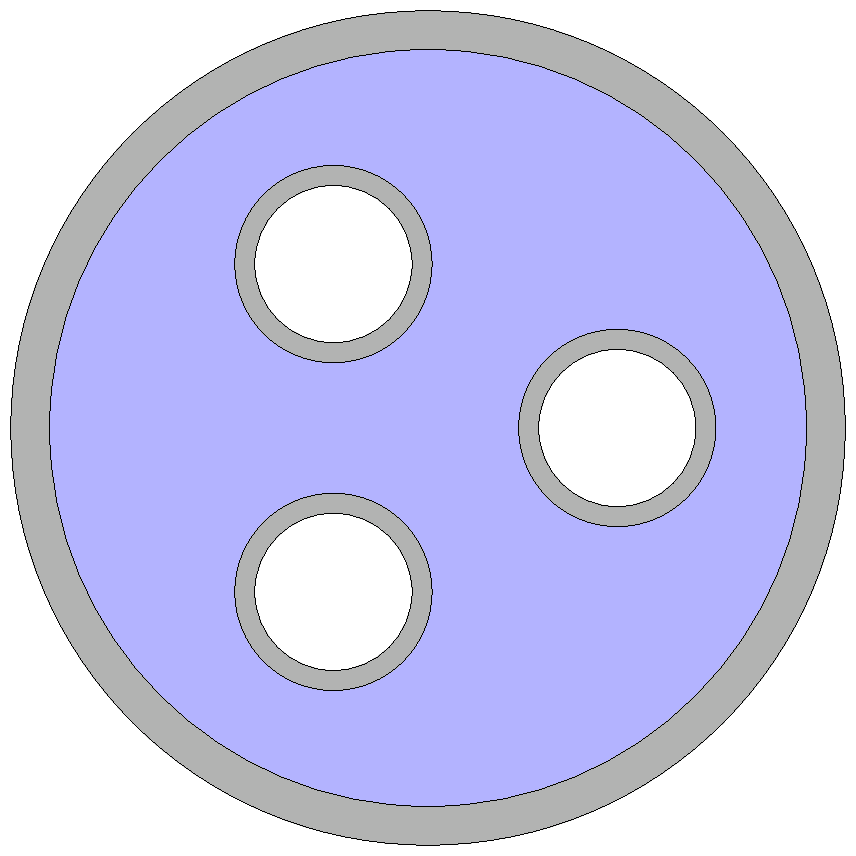
\includegraphics[width=2in]{imgs/ThreePipeHeatExchanger.pdf}

\begin{enumerate}

\item What is the Reynolds number for the flow?

\item What is the pressure drop across a length of 4 meters?

\end{enumerate}


\begin{solution}
\begin{align*}
    A &= 12910 - 3\times \pi/4(33.4)^2 = 12910 - 3\times 876.16 = 10282~\mm^2\\
    v&= \frac{800}{60000}\frac{1}{0.010282}=1.2968~\m/s\\
    WP &= \pi(128.2) + 3\times \pi(33.4)= 717.54~\mm \\
    D_h &= 4\times\frac{A}{WP}= 57.32~\mm \\
    N_R &=\frac{vD}{\nu} = \frac{1.2968 \times 0.05732}{1.15\times 10^{-6}}=64,637 = 6.5\times 10^4 \qquad{\rm (turbulent)}\\
    D/\epsilon &= \frac{0.05732}{4.6\times 10^{-5}}=1246\\
    f&=0.02264\\
    \Delta p&=\rho v^2/2 \times f \times L/D = 1000 (1.2968)^2/2 \times 0.02264\times 4/0.05732=1.15~\kPa
\end{align*}
\end{solution}

\end{question}






\begin{question}

Compute the volume flow rate of water through the pipe system shown below.
The piping is 4-in schedule 40 steel.

Take into account the following losses: entrance loss from the tank, a fully open gate valve, two ninety degree standard elbows, 85 feet of straight pipe, and loss through the nozzle.  Treat the nozzle as a sudden contraction from the 4-in pipe into a 2-in opening.

Report your volume flow rate in ft$^3$/s.

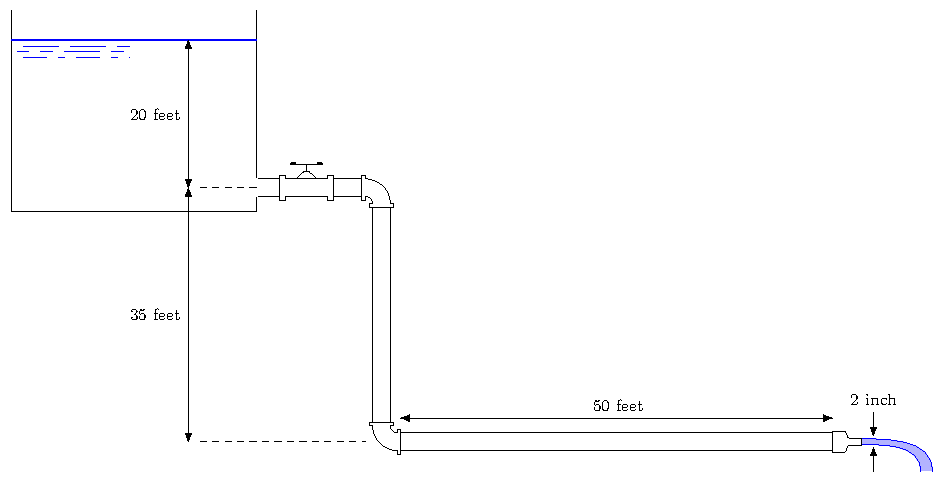
\includegraphics[width=5in]{imgs/TankGateElbows.pdf}


\begin{solution}

\end{solution}

\end{question}



\end{document}
